\documentclass{article}
\setlength\topmargin{0pt}
\addtolength\topmargin{-\headheight}
\addtolength\topmargin{-\headsep}
\setlength\oddsidemargin{0pt}
\setlength\textwidth{\paperwidth}
\addtolength\textwidth{-2in}
\setlength\textheight{\paperheight}
\addtolength\textheight{-2in}
\usepackage{layout}
\usepackage{amsmath}
\usepackage{algorithm}
\usepackage{verbatim}
\usepackage[noend]{algpseudocode}
\usepackage{graphicx}
\graphicspath{ {./} }


\title{\vspace{-2.0cm}CS M152A Project 3 Report}
\author{Melody Chen}

\begin{document}
\maketitle
\section{Introduction and Requirement} 
The focus of this lab is for students to learn to use the Xilinx ISE software to design and test various waveforms on a digital system. From the manual, we learned about basic concepts behind clocking a system and techniques to generate them from a system clock.  Clocks are very important for synchronous data transmission, allowing signals to be communicated between different devices. In this lab, we focus on creating clocks and pulses of different frequency and duty cycles, such as even division and odd division clocks. For this project, I designed and built many smaller sub-modules of individual types of clock, and combined them into one single \texttt{clock\_gen} top module to allow side-by-side comparisons of their waveforms and further analysis. All of my modules and sub-modules take system clock as an input in addition to a reset signal and outputs the derived clock. A brief summary of my top module and sub-modules are outlined below(from the project manual):
\begin{center}
    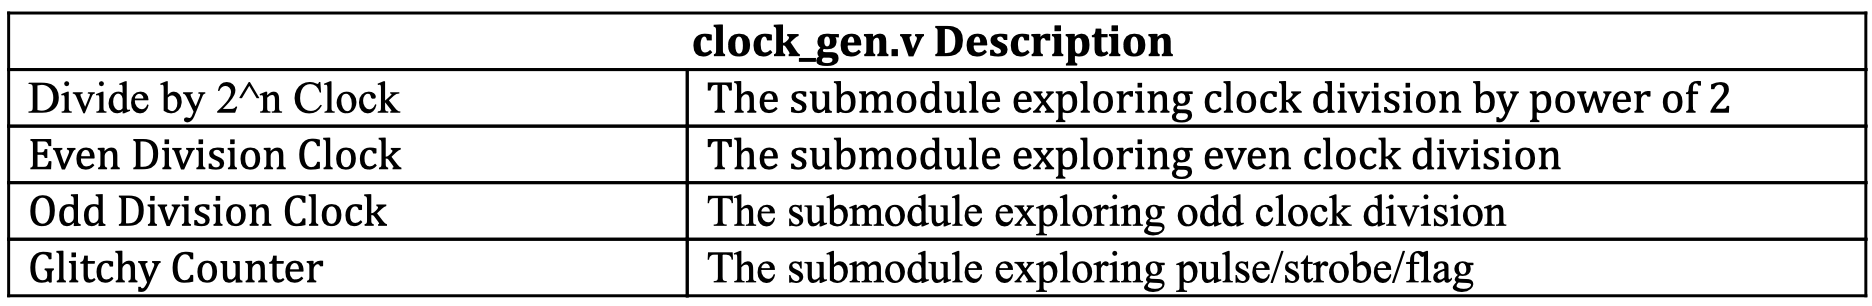
\includegraphics[scale=0.35]{intro.png} \\
    \caption{Outline of Top Module and Sub-modules}
\end{center}

\section{Design Description}
For the design and implementation of the varying types of clocks, I followed guidance provided in the project specifications. I designed and implemented a total of 7 sub-modules and 1 top modules that combines the sub-modules. Below, I will talk about my design and implementation of the modules based on the category of clocks it belongs to. In this project, we implement and work with the following categories of clocks: Clock Divider by Power of 2s, Even Division Clock Using Counters, Odd Division Clock Using Counters, Pulse/Strobes. All of my sub-modules take two inputs, the system clock \texttt{clk\_in} and reset signal \texttt{rst}. Output depends on each sub-module, but generally one or more derived clock signal will be outputted.
\renewcommand{\theenumi}{\alph{enumi}}
\begin{enumerate}
    \item \textbf{Category #1: } Clock Divider by Power of 2s \\
    In this category of clock, I designed one sub-module \texttt{clock\_div\_two} that outputs four clock signals: \texttt{clk\_div\_2}, \texttt{clk\_div\_4},  \texttt{clk\_div\_8}, and \texttt{clk\_div\_16}. I based my design of this sub-module on the 4-bit Counter I built for Project 1. The idea is to have a 4-bit register \texttt{Q[3:0]} that increments by 1 on each \texttt{posedge} of the clock. I then observe that the clock divider can be obtained by extracting the proper bit from the counter. Now, each bit represents a clock divider of a certain power of 2.  The LSB represents the \texttt{clk\_div\_2} signal, as its signal is 1 for every 2 \texttt{posedge} of the clock, thus it is twice as slow as the \texttt{clk\_in} signal. By the same logic, the 1st bit then represents the \texttt{clk\_div\_4} signal as the first bit changes signal from 0 to 1 every four clock cycles, so it is four times as slow as \texttt{clk\_in} signal. The same logic is applied to obtain the \texttt{clk\_div\_8} and \texttt{clk\_div\_16} signals. \par
    To implement this in Verilog, I replicate my 4-bit counter made in Project 1 which has an \texttt{always} block sensitive to the \texttt{posedge} of the clock signal. Inside, I increment register \texttt{Q[3:0]} by 1 unless \testtt{rst} is high. To extract each bit as a separate signal, I used four \texttt{assign} statements to assign each bit of \texttt{Q} to the corresponding output signal. \par
    The RTL schematic generated by the Xilinx ISE of my \texttt{clock\_div\_two} module is shown below. My Verilog code results in this schematic being generated as I used an adder to increment register \texttt{Q} and extracted the 4 bits as shown by the four wires to the right of the schematic.
    \begin{center}
    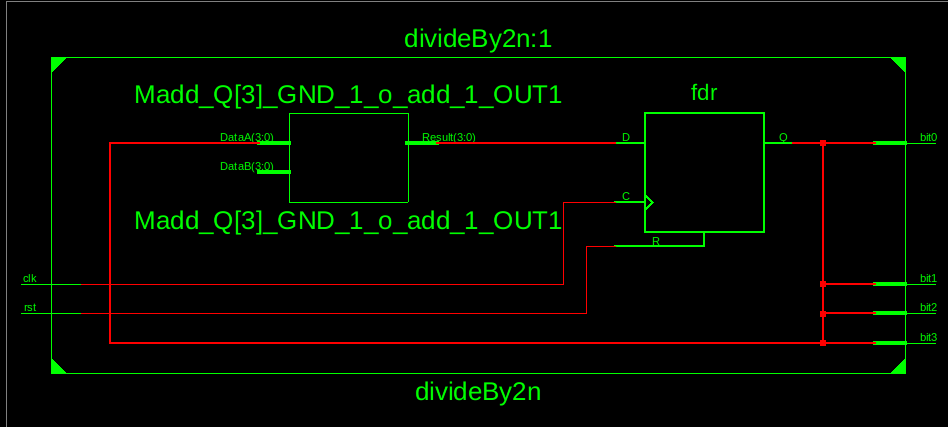
\includegraphics[scale=0.3]{rtl_div2.png} \\
    \caption{RTl Schematic of \texttt{clock\_div\_two} Module}
    \end{center} 
    
    \item \textbf{Category #2: } Even Division Using Counters \\
    In this category of clock, I designed two sub-modules that corresponds to two even division clock dividers: a divide-by-32 clock \texttt{clock\_div\_thirty\_two} module and a divide-by-28 clock \texttt{clock\_div\_} \texttt{twenty\_eight} module. For the \texttt{clock\_div\_thirty\_two} sub-module, I based my design again on the 4-bit counter, but instead of extracting bits, I check for overflow when the 4-bit register is incremented by 1. When overflow is detected which will be on the 16th \texttt{posedge}, our output clock signal will flip allowing us to have a output clock signal that is 32 times slower than the system clock. My design for the divide-by-28 clock \texttt{clock\_div\_twenty\_eight} module is then based off of this idea of detecting overflow. But since we want signal to flip on the 14th \texttt{posedge}, instead of detecting when the 4-bit register overflow as now we want a slightly faster clock, I detect when 4-bit register is 1 step before overflow, i.e. equal to \texttt{4'b1101}. This slight modification allows me to design a clock that is 28 times slower than the system clock. \par
    The implementation of these two sub-modules in Verilog is very similar. The  \texttt{clock\_div\_thirty\_two} module outputs signal \texttt{clk\_div\_32} and \texttt{clock\_div\_twenty\_eight} outputs signal \texttt{clk\_div\_28}. I have an \texttt{always} block sensitive to the \texttt{posedge} of the provided clock, and then I use if statements to detect when \texttt{rst} is high and when our 4-bit register \texttt{Q[3:0]} is equal to \texttt{4'b1111} for divide-by-32 or \texttt{4'b1101} for divide-by-28 clock. When \texttt{rst} is high, we reset \texttt{Q[3:0]} and our output clock signal to 0. When \texttt{Q} is equal to specified number \texttt{4'b1111} or \texttt{4'b1101}, we flip the output clock signal. \par
    The RTL schematic generated by the Xilinx ISE of my \texttt{clock\_div\_twenty\_eight} module is shown below. I chose to only show RTL schematic of one module in this category as the two implementations are very similar. My Verilog code results in this schematic being generated as I used an adder to increment register \texttt{Q}, a comparator to compare value of \texttt{Q} to specified number, and another register to store our output signal.
    \begin{center}
    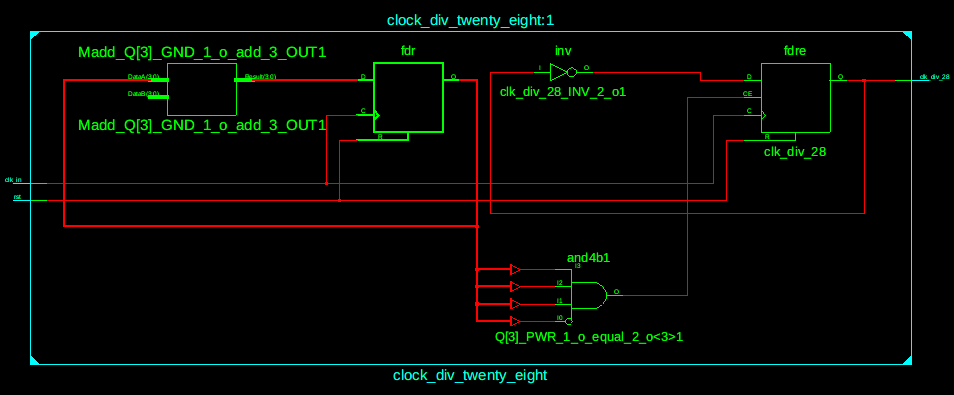
\includegraphics[scale=0.3]{rtl_div28.png} \\
    \caption{RTl Schematic of \texttt{clock\_div\_twenty\_eight} Module}
    \end{center} 
    
    \item \textbf{Category #3: } Odd Division Clock Using Counters \\
    In this category of clock, I designed two sub-modules that corresponds to the two tasks assigned: a 33\% duty cycle clock \texttt{clock\_div\_thirty\_three} module, and a divide-by-5 clock \texttt{clock\_div\_five} module. 33\% duty cycle clock means that for one third of a period it is 1 and 0 for the rest. To accomplish this, instead of using concept of 4-bit counter, I rotate a the 3-bit value \texttt{3'b100} to the left at each \texttt{posedge} and set the MSB as the output \texttt{clk\_div\_33} signal. This allows us to have a output clock signal that is 1 one-third of the time, as only 1 bit in \texttt{3'b100} is 1. To implement \texttt{clock\_div\_thirty\_three} module in Verilog, I used an \texttt{always} block sensitive to \texttt{posedge} of the system clock that uses concatenation to rotate our register \texttt{Q[2:0]} with initial value \texttt{3'b100} to the left. When \texttt{rst} is high, we reset \texttt{Q[2:0]} to \texttt{3'b100}. The MSB \texttt{Q[2]} is then assigned to output \texttt{clk\_div\_33} signal.   \par
    Following the task instructions, I duplicated another \texttt{always} block in the same module that is sensitive to \texttt{negedge} of the system clock. I created an extra output \texttt{clk\_div\_33\_neg} that holds the extra output. I assigned the logical \texttt{or} of \texttt{clk\_div\_33\_neg} and \texttt{clk\_div\_33} signal to \texttt{clk\_div\_33\_or} and observed that it is now a 50\% duty cycle divide-by-3 clock. With this idea, I can now design my divide-by-5 clock \texttt{clock\_div\_five} module with the same idea. Instead of \texttt{3'b100}, I rotate the value \texttt{5'b11000} because once I \texttt{or} the MSB from the output of \texttt{posedge} and \texttt{negedge}, I will have a 50\% duty cycle clock and it is a divide-by-5 clock because our rotated value is 5 bits which means our output clock signal will begin repeating after 5 clock cycles . \par
    The RTL schematic generated by the Xilinx ISE of my \texttt{clock\_div\_five} module is shown below. I chose to only show RTL schematic of one module in this category as the two implementations are very similar. My Verilog code results in this schematic being generated as I used two 5-bit registers \texttt{Q[4:0]} and \texttt{Q\_neg[4:0]}, and an or gate to get my final clock output.
    \begin{center}
    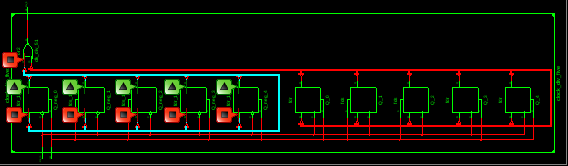
\includegraphics[scale=0.8]{rtl_div5.png} \\
    \caption{RTl Schematic of \texttt{clock\_div\_five} Module}
    \end{center} 
    
    \item \textbf{Category #4: } Pulses/Strobes \\
    For this clock category, I designed two sub-modules that corresponds to the three tasks assigned: a divide-by-200 clock using a divide-by-100 clock with 1\% duty cycle and \texttt{clock\_strobe} module that outputs a glitchy counter. To build the divide-by-100 clock with 1\% duty cycle, I used the same idea from building a 33\% duty cycle, but instead of rotating \texttt{3'b100}, I rotate \texttt{\{1'b1,\{99\{1'b0\}\}\}} stored in register \texttt{Q[99:0]} as we want clock to be 1 only 1\% of the time. The MSB is our output clock. To implement this in Verilog, I have one \texttt{always} block sensitive to \texttt{posedge} of system clock and it rotates \texttt{Q[99:0]} to the left each time. I assign \texttt{Q[99]} as output clock signal \texttt{clk\_div\_100}. \par
    Now, I want to use the divide-by-100 clock with 1\% duty cycle to create an output clock that is 50\% duty cycle divide-by-200 clock running at 500kHz. I can build this by adding an additional \texttt{always} block to my divide-by-100 clock module that flips the output clock \texttt{clk\_div\_200} every time \texttt{clk\_div\_100} signal is 1. With this our new output signal will flip every 100 system clock cycles, creating a 50\% duty cycle divide-by-200 clock that is 200x slower than system clock. Since system clock inputted is 100Mhz, our output clock will run 200x slower, resulting in $100MHz/200 = 500kHz$ output clock signal. \par
    Finally, we want to design our \texttt{clock\_strobe} module that generates an 8-but counter that counts up by 2 on every \texttt{posedge} of master clock and subtracts by 5 on every strobe. To detect when the strobes occur, I rotate the 4-bit value \texttt{4'b0001} stored in register \texttt{Q[3:0]} to the right on every \texttt{posedge} in the first \texttt{always} block. In another \texttt{always} block, I detect whether \texttt{Q[3]} is 1. If it is, I subtract 5 from 8-bit counter, if not, I add 2 to 8-bit counter. \par
    The RTL schematic generated by the Xilinx ISE of my \texttt{clock\_strobe} module is shown below. I chose to only show RTL schematic of one module in this category as the \texttt{clock\_div\_hundred} module is very similar to our previous modules. My Verilog code results in this schematic being generated as I used one 4-bit register \texttt{Q[3:0]} and the muxes represents the if statements in my \texttt{always} block to determine when to add 2 or subtract 5.
    \begin{center}
    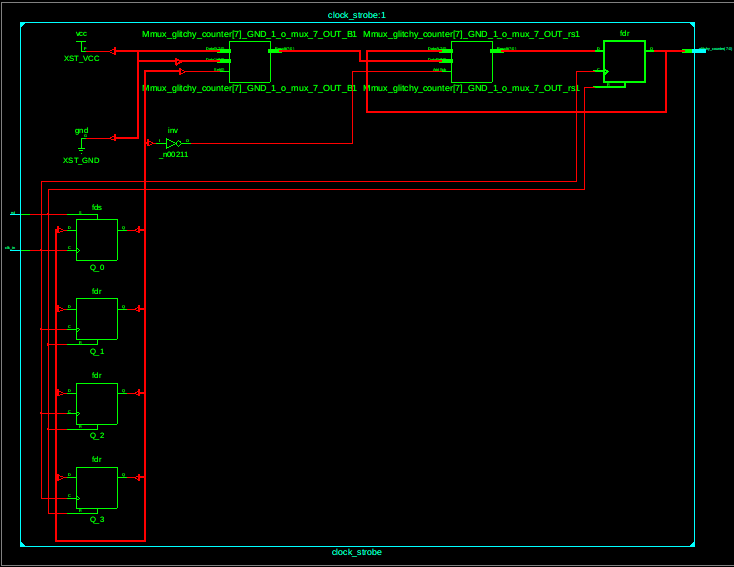
\includegraphics[scale=0.4]{rtl-strobe.png} \\
    \caption{RTl Schematic of \texttt{clock\_strobe} Module}
    \end{center} 
    
    \item \textbf{Top Module: }Clock Generator Module \\
    This module is the top module and combines the 4 deliverable tasks mentioned in the project manual. This top module takes the following inputs: input clock signal \texttt{clk\_in} and reset signal \texttt{rst}. It outputs the following clock signals: \texttt{clk\_div\_2}, \texttt{clk\_div\_4}, \texttt{clk\_div\_8}, \texttt{clk\_div\_16}, \texttt{clk\_div\_28}, \texttt{clk\_div\_5}, \texttt{[7:0] glitchy\_counter}. In this top module, I instantiated modules we previously built that provided us with the above outputs. The schematic of this module is not shown, as it is simply a combination of modules we previously described above.
\end{enumerate}

\section{Simulation Documentation}
To test whether the different types of clocks we designed for this project work as expected, I wrote separate test benches to produce waveforms for each module in addition to the test bench for the final clock generator module which combines many of the sub-modules we wrote. The test bench for all of my modules and final module looks very similar as all of the modules take two inputs: \texttt{clk\_in} and \texttt{rst}. In all my test benches, \texttt{rst} is only high in the very start to make sure all values are initialized correctly. Then, my \texttt{clk\_in} is flipped every certain amount of time depending on the module and the instructions.
\begin{enumerate}
    \item \textbf{(1)} Clock Divider by Power of 2s \\
    For the \texttt{clock\_div\_two} module, in my test bench I initially set \texttt{rst} to high and then flipped the \texttt{clk\_in} signal every 100ns. The resulting waveform is shown below. We can clearly observe that the \texttt{clk\_div\_2} clock signal is twice as slow as the \texttt{clk\_in}, because for two \texttt{clk\_in} cycles, we only observe one \texttt{clk\_div\_2} cycle. The same can be observed for the \texttt{clk\_div\_4}, \texttt{clk\_div\_8}, \texttt{clk\_div\_16} clock signals. For example, one \texttt{clk\_div\_16} cycle takes 16 \texttt{clk\_in}, showing that \texttt{clk\_div\_16} clock is 16 times slower than the provided clock signal. Thus, we observe that using counters, we can easily generate clocks that have periods that are even multiple of the original. 
    \begin{center}
        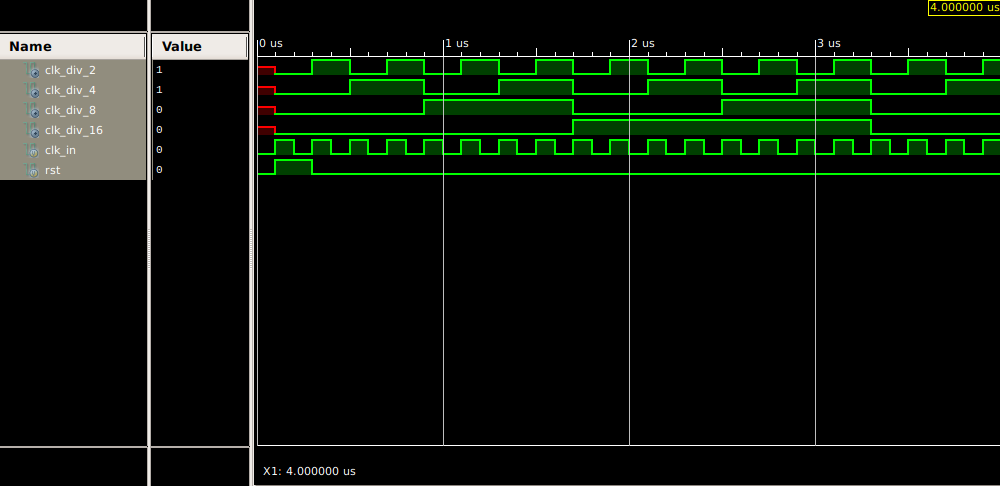
\includegraphics[scale=0.4]{waveform-1.png} \\
        \caption{\textbf{(1)} Simulation Waveform for \texttt{clock\_div\_two}}
    \end{center}
    \par
    
    \item \textbf{(2)} Divide-By-32 Clock \\
    For the \texttt{clock\_div\_thirty\_two} module, in my test bench I initially set \texttt{rst} to high and then flipped the \texttt{clk\_in} signal every 100ns. The resulting waveform is shown below. We can clearly observe that the \texttt{clk\_div\_32} signal is 32 times slower than the input \texttt{clk\_in} signal, so our module works as expected.
    \begin{center}
        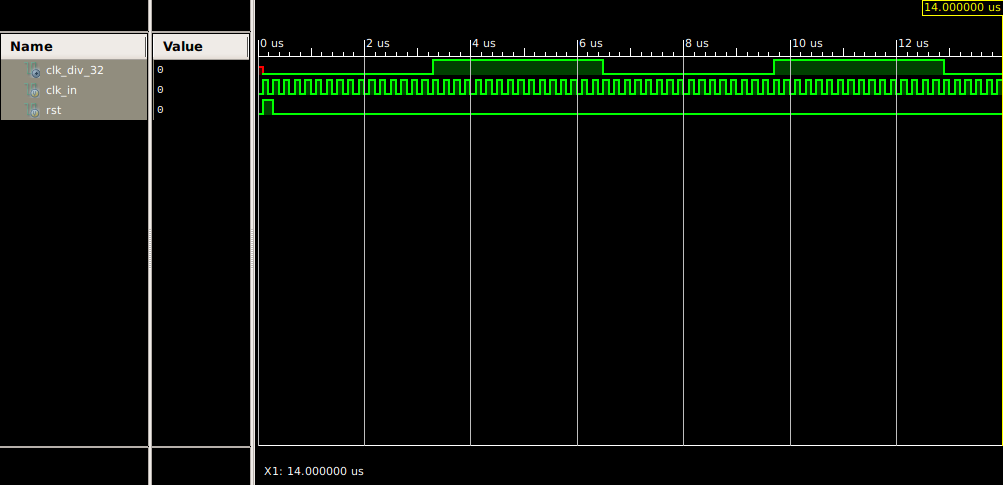
\includegraphics[scale=0.4]{waveform-2.png} \\
        \caption{\textbf{(2)} Simulation Waveform for \texttt{clock\_div\_thirty\_two}}
    \end{center}  \par

    \item \textbf{(3)} Divide-By-28 Clock  \\
    For the \texttt{clock\_div\_twenty\_eight} module, in my test bench I initially set \texttt{rst} to high and then flipped the \texttt{clk\_in} signal every 100ns. The resulting waveform is shown below. We can clearly observe that the \texttt{clk\_div\_28} signal is 28 times slower than the input \texttt{clk\_in} signal, so our module works as expected. One cycle of our \texttt{clk\_div\_28} clock signal takes 28 input clock cycles.
    \begin{center}
        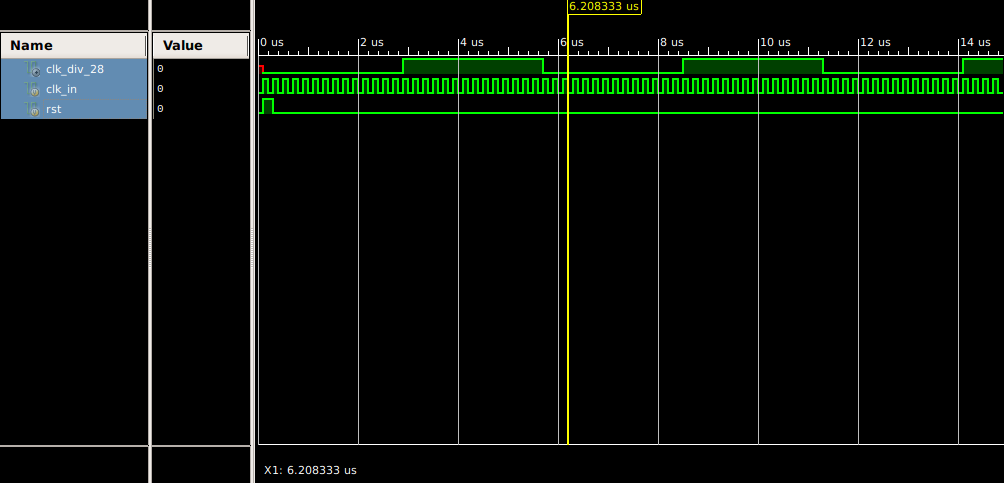
\includegraphics[scale=0.4]{waveform-3.png} \\
        \caption{\textbf{(3)} Simulation Waveform for \texttt{clock\_div\_twenty\_eight}}
    \end{center}
    \par
    
    \item \textbf{(4)} 33\% Duty Cycle Clock  \\
    For the \texttt{clock\_div\_thirty\_three} module, in my test bench I initially set \texttt{rst} to high and then flipped the \texttt{clk\_in} signal every 100ns. The resulting waveform is shown below. We can clearly observe that 1/3 of the time our output \texttt{clk\_div\_33} clock signal is 1 and the rest 2/3 of the time our output \texttt{clk\_div\_33} clock signal is 0. To illustrate, we can observe for one cycle of \texttt{clk\_in}, \texttt{clk\_div\_33 = 1} and following that cycle for two cycles of \texttt{clk\_in}, \texttt{clk\_div\_33 = 0}.
    \begin{center}
        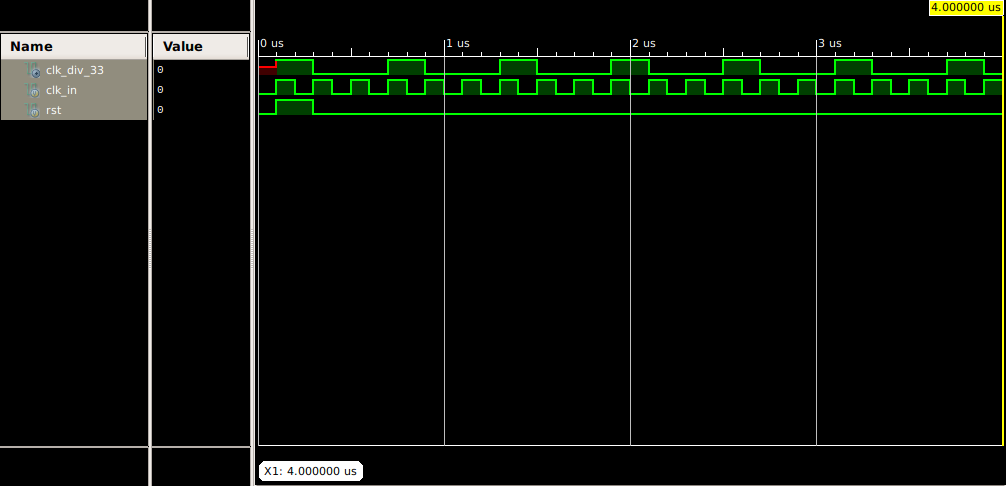
\includegraphics[scale=0.4]{waveform-4.png} \\
        \caption{\textbf{(4)} Simulation Waveform for \texttt{clock\_div\_thirty\_three}}
    \end{center}

    \item \textbf{(5)} Side by Side 33\% Duty Cycle Clock  \\
    For this task, we build on the \texttt{clock\_div\_thirty\_three} module, by adding an \texttt{always} block sensitive to \texttt{negedge} of the clock. Side by side waveform of the two output clock signals is shown below. We can observe that the \texttt{clk\_div\_33\_neg} signal is half a cycle behind the \texttt{clk\_div\_33} as it is sensitive to the negative edge of the clock.
    \begin{center}
        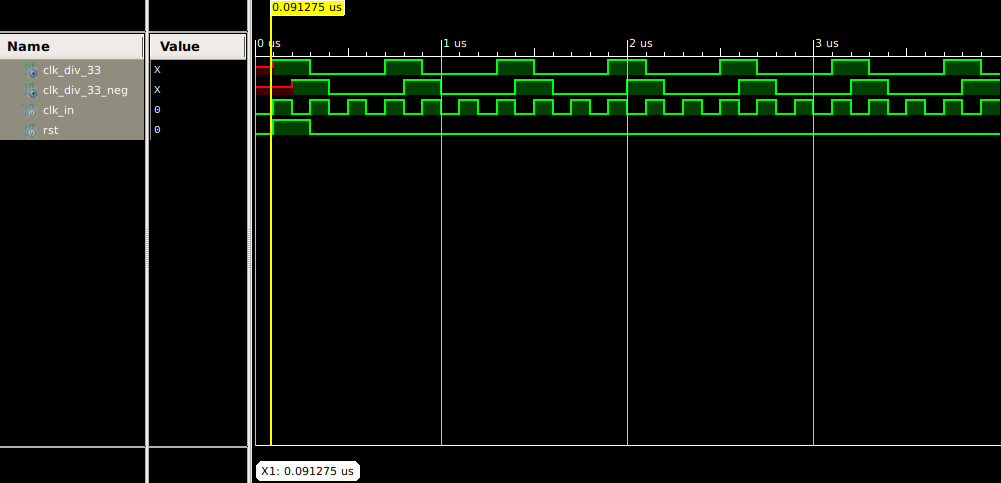
\includegraphics[scale=0.4]{waveform-5.png} \\
        \caption{\textbf{(5)} Simulation Waveform for \texttt{clock\_div\_thirty\_three} Side by Side}
    \end{center}
    
    \item \textbf{(6)} Logical Or of two 33\% Duty Cycle Clock  \\
    For this task, we build on the \texttt{clock\_div\_thirty\_three} module with addition of an \texttt{always} block sensitive to \texttt{negedge} of the clock and logical or the two outputs \texttt{clk\_div\_33} and \texttt{clk\_div\_33\_neg} to get \texttt{clk\_div\_33\_or} signal. The resulting waveform is shown below. We can observe that the \texttt{clk\_div\_33\_or} signal is actually a 50\% duty cycle divide-by-3 clock.
    \begin{center}
        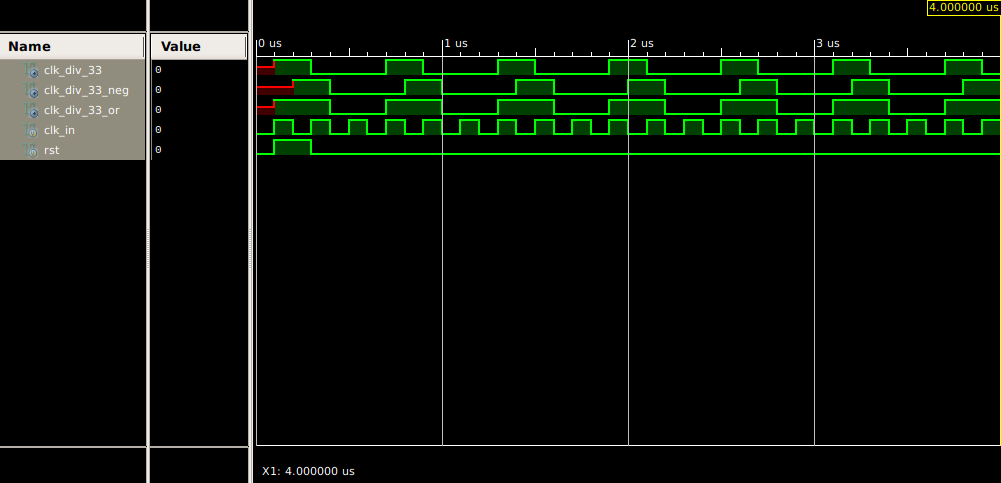
\includegraphics[scale=0.4]{waveform-6.png} \\
        \caption{\textbf{(6)} Simulation Waveform for \texttt{clock\_div\_thirty\_three} Logical Or}
    \end{center}
    
    \item \textbf{(7)} 50\% Duty Cycle Divide-By-5 Clock  \\
    For this task, we built the \texttt{clock\_div\_five} module. In my test bench for this module, I initially set \texttt{rst} to high and then flipped the \texttt{clk\_in} signal every 100ns. The resulting waveform is shown below. We observe that for five cycles of the input clock, we have one cycle for our output \texttt{clk\_div\_5} clock signal, showing that our module works as expected and produces a clock that is five times slower than the input clock.
    \begin{center}
        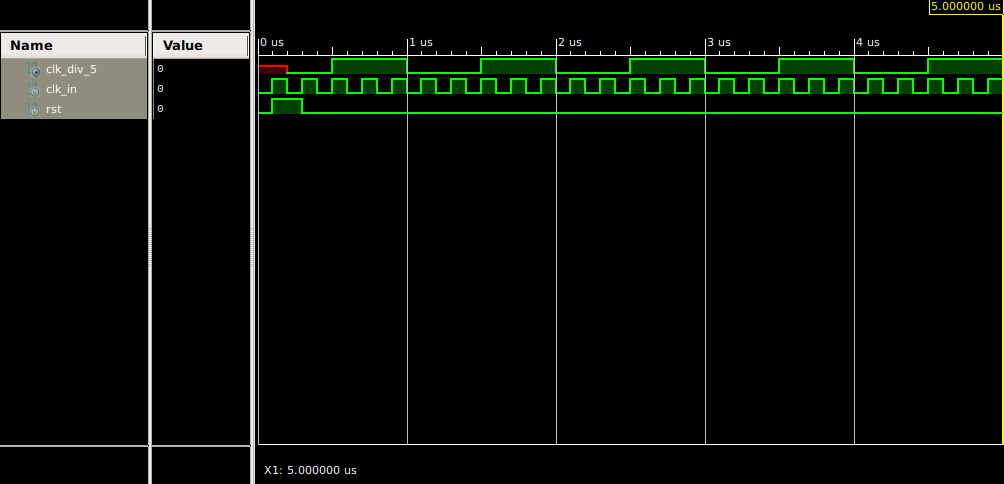
\includegraphics[scale=0.4]{waveform-7.png} \\
        \caption{\textbf{(7)} Simulation Waveform for \texttt{clock\_div\_five}}
    \end{center}
    
    \item \textbf{(8)} 50\% Duty Cycle Divide-By-200 Clock at 500kHz  \\
    For this task, we built the \texttt{clock\_div\_two\_hundred} module. In my test bench for this module, I initially set \texttt{rst} to high and then flipped the \texttt{clk\_in} signal every 5ns to create a 100Mhz system clock. The resulting waveform is shown below. We observe that our output clock signal \texttt{clk\_div\_200} has period of 2us. Since it has a period of 2us, this means that the frequency of our \texttt{clk\_div\_200} clock is $1/0.000002s = 500kHz$, which matches the description in the project manual. This also makes sense as our output clock signal should be 200x slower then the input system clock, $100mHz/200 = 500kHz$. It is also clearly a 50\% duty cycle clock as half of the period, our output clock signal is 1. 
    \begin{center}
        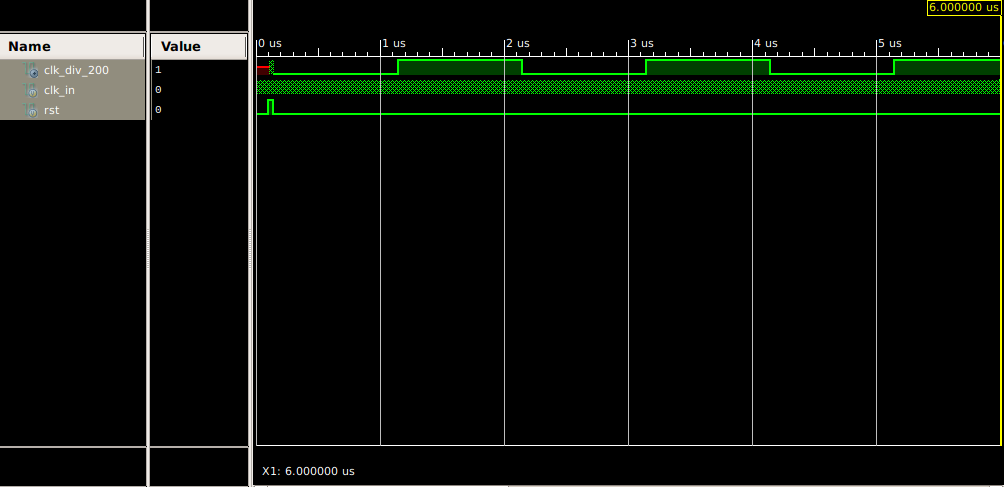
\includegraphics[scale=0.4]{waveform-8.png} \\
        \caption{\textbf{(8)} Simulation Waveform for \texttt{clock\_div\_two\_hundred}}
    \end{center}
    One bug I found during simulation for this module is that initially the period of \texttt{clk\_div\_200} clock is 8us instead of the expected 2us. Because of this, I went back to investigate my Verilog code and realize that I had calculated my input system clock's value incorrectly and was able to fix the system clock's frequency. 
    \item \textbf{(9)} Glitchy Counter \\
    For this task, we built the \texttt{clock\_strobe} module. In my test bench for this module, I initially set \texttt{rst} to high and then flipped the \texttt{clk\_in} signal every 100ns. The resulting waveform is shown below. We observe that our glitchy counter's output correctly counts up by 2 on every positive edge of the master clock, and subtracts by 5 on every strobe. 
    \begin{center}
        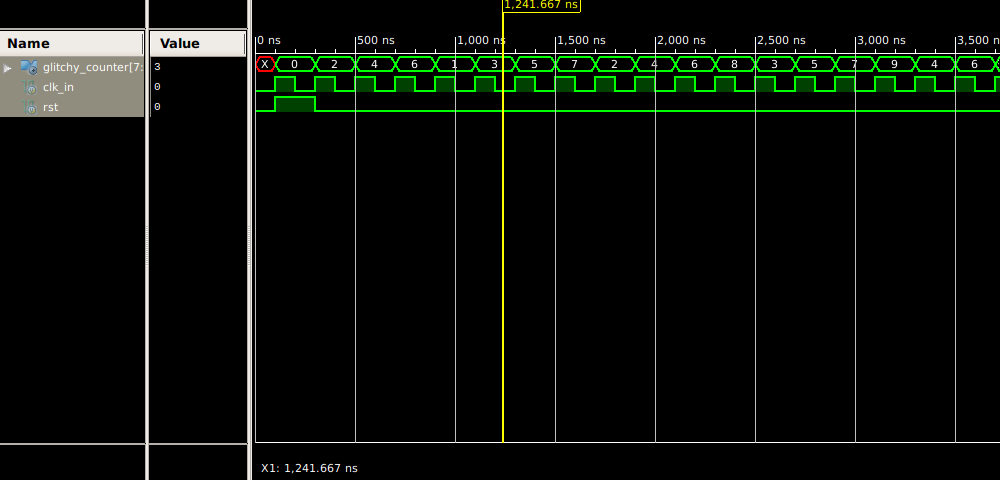
\includegraphics[scale=0.4]{waveform-9.png} \\
        \caption{\textbf{(9)} Simulation Waveform for \texttt{clock\_strobe}}
    \end{center}
    
    \item \textbf{(10)} Clock Generator Module \\
    The Clock Generator Module \texttt{clock\_gen} combines our sub-modules together, so we can observe different types of clocks all in one wave form.  In my test bench for this module, I initially set \texttt{rst} to high and then flipped the \texttt{clk\_in} signal every 20ns. The resulting waveform is shown below.
    \begin{center}
        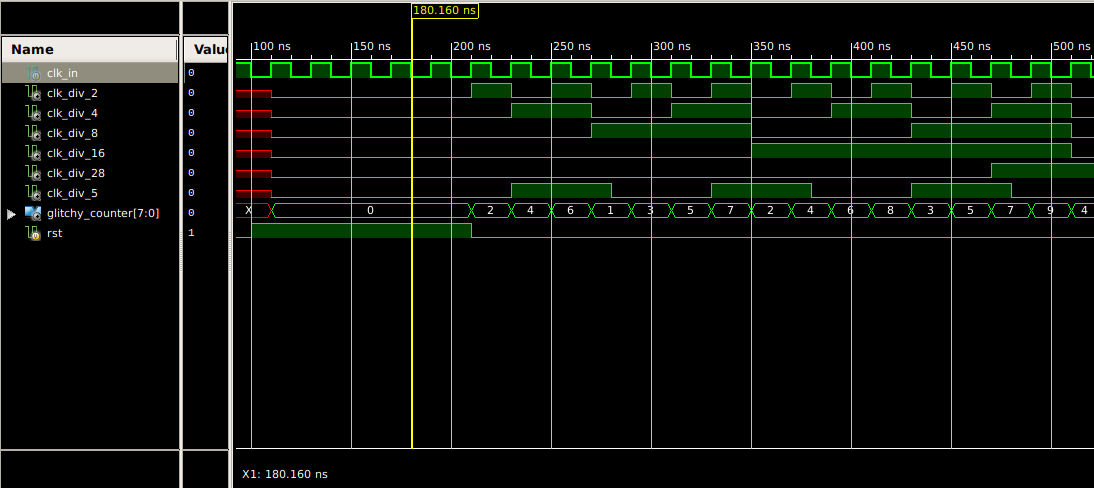
\includegraphics[scale=0.4]{waveform-10.png} \\
        \caption{\textbf{(10)} Simulation Waveform for \texttt{clock\_gen}}
    \end{center}
\end{enumerate}

\section{Conclusion} 
In this project, I designed and implemented clocks and pulses of different frequency and duty cycles. They were designed based on ideas formulated in Project 1 and hints provided in the project manual. The even division clocks were relatively easier to implement than odd division clocks, as even division clock's implementation simply involves using counters of various bits. The main idea I used for odd division clock was rotating a binary value of certain length with varying number of 1's and 0's. For the glitchy counter module, I combined ideas from both even and odd division clock. \par
Some difficulties I encountered include coming up with the initial idea of how to build an odd division clock. But, with the help of the TA's lab section, I was able to come up with the correct idea, experiment with Verilog code, and eventually come up with a working implementation. Another difficulty I encountered was interpreting the RTL schematic generated by Xilinx ISE. I dealt with this by investigating closely the purpose of each component and looking through the Xilinx documentation.



\end{document}